\documentclass[a4paper,11pt]{article}%Schriftgröße
\usepackage[T1]{fontenc} 
\usepackage[utf8]{inputenc}
\usepackage[ngerman]{babel}%Veröffentlichungssprache
\usepackage{graphicx}
\usepackage{ragged2e}
\usepackage[format=plain,justification=RaggedRight,singlelinecheck=false,font={small},labelsep=space]{caption}
\usepackage{xcolor}	
\usepackage[a4paper]{geometry}
	\geometry{left=3.5cm,right=2.5cm,top=2.4cm,bottom=2cm}%Seitenränder
	\usepackage[onehalfspacing]{setspace}%Zeilenabstand
	\renewcommand{\\}{\vspace*{0.5\baselineskip} \newline}
\renewcommand*\MakeUppercase[1]{#1}	
\usepackage{fancyhdr}
	\pagestyle{fancy}
	\renewcommand{\headrulewidth}{0pt}
	\renewcommand{\footrulewidth}{0pt}
	\fancyhead[R]{\footnotesize{\thepage}}
	\fancyhead[L]{\footnotesize{\leftmark}}
	\fancyfoot{}
\usepackage[colorlinks,
pdfpagelabels,
pdfstartview = FitH,
bookmarksopen = true,
bookmarksnumbered = true,
linkcolor = black,
urlcolor = black,
plainpages = false,
hypertexnames = false,
citecolor = black] {hyperref}
	
\begin{document}
\begin{titlepage}
\begin{flushleft}
	\vspace*{-1cm}
	
\includegraphics[scale=1]{Grafiken/TH.png}\\
	\vspace*{1cm}
\end{flushleft}
\begin{huge}
	\noindent
	Effizientes und realistisches Partikelsystem zur \newline 
	Simulation von Feuer und Rauch in VR-Umgebung \\
\end{huge}
Bachelorarbeit zur Erlangung des Bachelorgrades \newline
Bachelor of Science im Studiengang Medientechnologie \newline
an der Fakultät für Informations-, Medien- und Elektrotechnik \newline
der Technischen Hochschule Köln \\
~\\
~\\
~\\
\noindent\begin{tabular}{ll}
	vorgelegt von: & Miro Steiger \\
	Matrikel-Nr.: &	111 212 81 \\
	Adresse: & Venloer Straße 202 \\
	~ &	50823 Köln \\
	~ &	miro.steiger@smail.th-koeln.de \\
	~ & ~ \\
	eingereicht bei: & Prof. Dr.-Ing. Arnulph Fuhrmann \\
	Zweitgutachter: & Prof. Dr. rer. nat. Stefan Michael Grünvogel 
\end{tabular}	
~\\
~\\
Köln, TT.MM.JJJJ
\end{titlepage}
\pagenumbering{Roman}
\pagestyle{fancy}
\newpage
\section*{Erklärung}\markboth{Erklärung}{Erklärung}\addcontentsline{toc}{section}{Erklärung}
Ich versichere, die von mir vorgelegte Arbeit selbstständig verfasst zu haben. Alle Stellen, die wörtlich oder sinngemäß aus veröffentlichten oder nicht veröffentlichten Arbeiten anderer oder der Verfasserin/des Verfassers selbst entnommen sind, habe ich als entnommen kenntlich gemacht. Sämtliche Quellen und Hilfsmittel, die ich für die Arbeit benutzt habe, sind angegeben. Die Arbeit hat mit gleichem Inhalt bzw. in wesentlichen Teilen noch keiner anderen Prüfungsbehörde vorgelegen.\\
Anmerkung: In einigen Studiengängen steht die Erklärung am Ende des Textes.\\
~\\
~\\
\rule{0.35\textwidth}{0.4pt} \hspace*{3cm} \rule{0.45\textwidth}{0.4pt} \newline
Ort, Datum	\hspace*{6.3cm}	Rechtsverbindliche Unterschrift
\newpage
\section*{Kurzfassung/Abstract}\markboth{Kurzfassung/Abstract}{Kurzfassung/Abstract}\addcontentsline{toc}{section}{Kurzfassung/Abstract}
Eine Kurzfassung (wenn verlangt) in Deutsch und/oder in Englisch (Abstract) umfasst auf etwa 1/2 bis 1 Seite die Darstellung der Problemstellung, der angewandten Methode(n) und des wichtigsten Ergebnisses.\\
Wie man ein gelungenes Abstract verfasst, erfahren Sie in den \href{https://www.th-koeln.de/studium/schluesselkompetenzen_25490.php}{\underline{Seminaren des Akademischen} \underline{Schreibzentrums der Kompetenzwerkstatt}}.\\
Schlagwörter/Schlüsselwörter: evtl. Angabe von 3 bis 10 Schlagwörtern 
\newpage
\tableofcontents
\newpage
\listoftables\addcontentsline{toc}{section}{Tabellenverzeichnis}
\newpage
\listoffigures\addcontentsline{toc}{section}{Abbildungsverzeichnis}
\newpage
\pagenumbering{arabic}
\section*{Einleitung}\markboth{Einleitung}{Einleitung}\addcontentsline{toc}{section}{Einleitung}
Hier kommt die Einleitung hin.

\subsection*{Problemanalyse}
\subsection*{Zielsetzung}

\newpage
\section{Formaler Aufbau}
\subsection{Reihenfolge}
Eine wissenschaftliche Arbeit besteht in der Regel aus den folgenden Teilen:
\begin{enumerate}
	\item Deckblatt
	\item Erklärung (auch am Ende üblich)
	\item Kurzfassung/Abstract (optional)
	\item Inhaltsverzeichnis
	\item Abbildungs- und Tabellenverzeichnis (auch am Ende üblich)
	\item Abkürzungsverzeichnis (auch am Ende üblich)
	\item Einleitung
	\item Hauptteil
	\item Zusammenfassung/Fazit
	\item Literaturverzeichnis
	\item Anhänge (optional)
\end{enumerate}
\subsection{Deckblatt}	
Die Gestaltung des Deckblatts folgt den visuellen Vorgaben für Publikationen der TH Köln.\\
Das Deckblatt beinhaltet: Art der Arbeit, Titel der Arbeit, Verfasser/in, Matrikelnummer, Abgabetermin, Betreuer/in sowie Zweitgutachter/in. Das Deckblatt wird bei Arbeiten über 15 Seiten bei der Seitenanzahl mitgezählt, jedoch nie nummeriert.

\subsection{Inhaltsverzeichnis}
Die Gliederung wird durch \LaTeX~selbst vorgenommen, wobei die oberste Gliederungsebene \textbackslash\textit{section} ist und die unterste \textbackslash\textit{subsubsection}. Alle drei Gliederungsebenen werden automatisch im Inhaltsverzeichnis aufgeführt. \\
Ist eine tiefere Gliederung notwendig, lassen sich mit den Befehlen \textbackslash\textit{paragrapgh} und \textbackslash\textit{subparagraph} weitere unnummerierte Gliederungsebenen, welche nicht im Inhaltsverzeichnis aufgeführt werden, einfügen.\\
Für eine Abschlussarbeit ist eine Gliederungstiefe von wenigstens drei Ebenen üblich. Hier sollten Sie aber unbedingt die Gepflogenheiten in Ihrem Fach erfragen.\\
Werden innerhalb eines Kapitels Unterüberschriften verwendet, müssen mindestens zwei vorhanden sein: wo ein 2.1 ist, muss es ein 2.2 geben.

\subsection{Abbildungsverzeichnis und Tabellenverzeichnis}
Abbildungen und Tabellen werden in entsprechenden Verzeichnissen gelistet. In dieser Vorlage erscheinen sie direkt nach dem Inhaltsverzeichnis. Dann können die entsprechenden Seiten römisch gezählt werden. Die Verzeichnisse können jedoch auch am Ende der Arbeit vor dem Literaturverzeichnis stehen. Dafür müssen die Quellcodezeilen 83-86 ans Ende der Datei verschoben werden. In dem Fall werden sie regulär mit Seitenzahlen versehen. Verzeichnisüberschriften (Abbildungsverzeichnis) werden nie nummeriert. \\
Sowohl Abbildungen als auch Tabellen werden in Gleitumgebungen angegeben, versieht man sie mit dem korrekten Befehl (siehe 2.6), legt sich das Abbildungs- und Tabellenverzeichnis selbstständig an. 

\subsection{Abkürzungsverzeichnis}
Die Zahl der Abkürzungen sollte übersichtlich bleiben. Das Abkürzungsverzeichnis enthält lediglich wichtige fachspezifischen Abkürzungen in alphabetischer Reihenfolge, insbesondere Abkürzungen von Organisationen, Verbänden oder Gesetzen. Gängige Abkürzungen wie u.a., z.B., etc. werden nicht aufgenommen.

\subsection{Literaturverzeichnis}
Das Literaturverzeichnis wird alphabetisch nach Autorennamen geordnet. Es enthält alle im Text zitierten Quellen und nur diese. Mehrere Schriften einer Person werden nach Erscheinungsjahr geordnet. Schriften derselben Person aus einem Erscheinungsjahr müssen Sie selbst unterscheidbar machen. Mehr hierzu im Online-Lernmodul \href{https://ilias.th-koeln.de/ilias.php?baseClass=ilRepositoryGUI}{\underline{Zitierwissen kompakt}}.\\
In den Ingenieurwissenschaften wird zusätzlich häufig ein Nummern- oder Autorenkürzel dem Namen in eckigen Klammern vorangestellt. Auch hierzu mehr im Lernmodul.\\
Die Quellen werden am Ende des Codes in der \textit{thebibliography}-Umgebung angeben und im Text mit dem zugehörigen Befehl aufgerufen (siehe 3.1). Das Literaturverzeichnis erstellt sich dann von selbst, zur Verwaltung der verwendeten Literatur eignet sich Citavi.

\subsection{Rechtschreibung, Grammatik}
Achten Sie bei der Abgabe Ihrer Arbeit auf ein einwandfreies Deutsch bzw. Englisch. Wenn Fehler die Lesbarkeit beeinträchtigen, kann sich dies sogar negativ auf die Note auswirken. \TeX -studio zeigt Rechtschreibfehler im Code unmittelbar an, die Sprache lässt sich über \textit{Optionen} verändern.\\
Für alle, die sich bei diesem Thema unsicher fühlen, empfehlen wir die Selbstlernmodule \href{https://ilias.th-koeln.de/ilias.php?baseClass=ilRepositoryGUI}{\underline{Rechtschreibung}} und \href{https://ilias.th-koeln.de/ilias.php?baseClass=ilRepositoryGUI}{\underline{Zeichensetzung}} des Akademischen Schreibzentrums. Wenden Sie sich gegebenenfalls auch an die \href{https://www.th-koeln.de/personen/nadine.sohn/}{\underline{Beauftragte für Studierende mit Beeinträchtigung}}.

\subsection{Umfang der Arbeit}
Alle Fächer nennen verbindliche Angaben zu Unter- und Obergrenzen, die in der Regel eingehalten werden müssen. Verzeichnisse und Anhänge werden dabei nie mitgezählt. In Einzelfällen – insbesondere bei empirischen Arbeiten – können abweichende Vereinbarungen mit der Betreuungsperson getroffen werden.

\section{Gestaltung}
\subsection{Seiteneinrichtung}
\textit{Papierformat}: DIN A4, Hochformat, einspaltig \\
\textit{Layout:} Die Dokumentvorlage ist so angelegt, dass jedes Blatt nur auf der Vorderseite bedruckt wird. \\
\textit{Seitenränder:} oben 2,4 cm; unten 2,0 cm; links 3,5 cm (wegen der Bindung); rechts (Korrekturrand) in der Regel 2,5 cm, bitte Fachvorgaben beachten. Eingestellt wird dies in Codezeile 10.

\subsection{Seitennummerierung}
Diese Dokumentvorlage verwendet die Variante mit römischen und arabischen Ziffern: Hier werden alle Teile nach dem Deckblatt und vor dem Textteil (d.h. Erklärung, evtl. Vorwort, evtl. Kurzfassung/Abstract, Inhaltsverzeichnis, evtl. Abbildungs-/Tabellenverzeichnis, evtl. Abkürzungsverzeichnis) seitenweise mit römischen Ziffern paginiert und die Seiten ab dem Textteil mit arabischen Ziffern.\\
Auch hier sind die Regelungen nicht einheitlich. Häufig beginnt die Durchnummerierung der Seiten direkt nach dem Deckblatt mit Seite 2. Hierfür verantwortlich ist der Befehl \textbackslash\textit{pagenumbering}\{\} (siehe Codezeile 65).\\
Die Seitenzahlen können entweder unten mittig oder oben rechts platziert werden, nie jedoch auf dem Deckblatt. Die zugehörigen Einstellungen sind mit dem \textit{fancyhdr-Paket} in der Präambel festgelegt (siehe ab Codezeile 14).

\subsection{Kopfzeile}
Diese Vorlage wurde so eingerichtet, dass die aktuelle Überschrift eines Kapitels (Ebene 1) immer korrekt in den Kopfzeilen der entsprechenden Seiten angezeigt wird. Die zugehörigen Einstellungen sind mit dem \textit{fancyhdr-Paket} in der Präambel festgelegt (siehe ab Codezeile 14).

\subsection{Format der Quellenangaben}
Quellenangaben können je nach Zitierstil als Fußnoten, als Endnoten oder als Kurzverweis im laufenden Text erscheinen. Die Wahl des richtigen Zitierstils hängt immer von Ihrer Fächergruppe, nicht selten sogar von den jeweiligen Prüfenden ab. Sie sollten sich gründlich über das richtige Zitieren in Ihrem Fach informieren. Wir empfehlen hierfür das Online-Lernmodul \href{https://ilias.th-koeln.de/ilias.php?baseClass=ilRepositoryGUI}{\underline{Zitierwissen kompakt}} des Akademischen Schreibzentrums.

\subsection{Schrift}
Die Schriftart im vorliegenden Dokument ist die in \LaTeX~verwendete Standardschriftart und heißt Computer Modern Schriftfamilie, die Schriftgröße beträgt 11 (siehe Codezeile 1). Es gibt zur Zeit mehr als 100 frei verfügbare Schriftarten für \LaTeX, unter anderem auch eine Arial-ähnliche Schrift. Das einbinden einer anderen Schriftart passiert in der Präambel des Dokuments. Die Schriftgröße sollte immer zwischen 10,5 und 12 Punkt liegen. \\
Der Zeilenabstand sollte auf mehrfach: 1,3 bis 1,5-fach eingestellt sein; hier beträgt er 1,5. Die Textausrichtung ist Blocksatz im Textteil und linksbündig in den Verzeichnissen.

\subsection{Abbildungen und Tabellen}
Grafiken und Tabellen müssen leicht verständlich und gut lesbar sein. Dafür ist es wichtig, dass die übliche Leserichtung von oben nach unten und von links nach rechts auch in der Darstellung berücksichtigt wird.
\begin{figure}[h]
	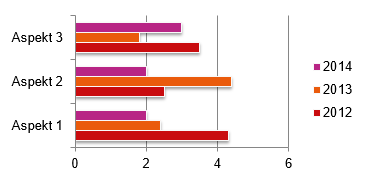
\includegraphics[scale=0.9]{Grafiken/Abbildung1.png}\\
	\begin{footnotesize}
		\caption[Abbildung 1]{Entwicklung seit 2006}
	\end{footnotesize}
\end{figure}
~\newline Mit \LaTeX~lassen sich Abbildungs- und Tabellenverzeichnisse automatisch erstellen. Dazu müssen die Tabellen und Abbildungen in \textit{Gleitumgebungen} angegeben und mit dem korrekten Befehl versehen werden: \\
Das Öffnen einer \textit{Gleitumgebung} für Grafiken geschieht mittels \textbackslash\textit{begin}\{\textit{figure}\}[h]... \textbackslash\textit{end}\{\textit{figure}\}, einer für Tabellen mittels \textbackslash\textit{begin}\{\textit{table}\}[h]... \textbackslash\textit{end}\{\textit{table}\}. Das [h] sorgt dafür, dass die Umgebung an genau der Stelle, an der Sie auch im Quellcode steht, platziert wird. Wird in der \textit{Gleitumgebung} der Befehl \textbackslash\textit{caption}[\textit{Hier steht der Name aus dem Verzeichnis}]\{\textit{Hier steht die Bildunterschrift}\} angegeben, wird automatisch ein Eintrag im Abbildungs- oder Tabellenverzeichnis erstellt.
\begin{table}[h]
	\renewcommand*{\arraystretch}{2}
	\setlength{\tabcolsep}{1.5cm}
	\begin{tabular}{lll}
		\hspace{-1.5cm}\textbf{Überschrift 1} & \textbf{Überschrift 2} & \textbf{Überschrift 3}\\ \hline
		\hspace{-1.5cm}ABC &	123 & 456 \\ \hline
		\hspace{-1.5cm}DEF &	414 & 63 \\ \hline
	\end{tabular}
	\caption[Tabelle 1]{Mustertabelle}
\end{table}
~\newline
In dieser Vorlage sind Tabellen und Abbildungen fortlaufend nummeriert. Auf jede Abbildung und jede Tabelle muss im Text verwiesen werden.

\section{Zitate und Literaturangaben}
Fremdes Gedankengut muss immer kenntlich gemacht werden. Vor allem muss es überprüfbar und auffindbar sein. Hierzu dient die Technik des Zitierens und Belegens.\\
Jede Fachrichtung und manchmal jeder Studiengang folgt spezifischen Zitierkonventionen. Sie finden sie im Kapitel Zitierstile im ILIAS-Lernmodul \href{https://ilias.th-koeln.de/ilias.php?baseClass=ilRepositoryGUI}{\underline{Zitierwissen kompakt}} des Akademischen Schreibzentrums, das laufend aktualisiert wird.

\subsection{Zitieren}
Bitte legen Sie den Zitierstil immer am Anfang fest und wechseln sie ihn nicht.\\
Wörtlich übernommene Textpassagen werden durch Anführungszeichen unten und oben (\glqq...\grqq) kenntlich gemacht, ein Beispiel ist an dieser Stelle im Quellcode zu finden. Die Anführungszeichen müssen mit Hilfe eines Befehls angegeben werden, gewöhnlichen Anführungszeichen führen bei \LaTeX~zu Sonderzeichen.\\
Wenn Ihr Zitat bereits ein Zitat enthält, müssen Sie die doppelten Anführungszeichen im Text durch einfache Anführungszeichen ersetzen (\glq...\grq), ein Beispiel ist an dieser Stelle im Quellcode zu finden. Auch diese müssen mit Hilfe eines Befehls angegeben werden.\\
In \LaTeX~funktioniert das Zitieren\cite[Beispielzitat aus Quelle 7]{FN} mit Hilfe des Befehls \textbackslash\textit{cite}.

\subsubsection{Quellenverweise}
Für alle Zitate muss ein Quellenverweis erstellt werden. Der Quellenverweis ist eine in der Form festgelegte Kurznotation, die auf die vollständige Literaturangabe im Literaturverzeichnis verweist. Quellenverweise können \textit{entweder} im laufenden Text (angloamerikanische Zitierweise bzw. Harvard-Stil) oder über eine Fußnote am unteren Ende der Seite oder in einer Endnote am Ende des gesamten Textes erfolgen. Hier gelten unterschiedliche fachliche Konventionen, die unbedingt beachtet werden müssen.\\
Entscheidet man sich für Kurzverweise im Textfluss oder für Endnoten, kann der Fußnotenbereich für Kommentare und für Verweise auf Stellen im eigenen Text genutzt werden.\\
\textit{Beachten Sie die Positionen von Hochzahl und Satzpunkten:}\\ 
Wenn das wörtliche Zitat selbst mit einem Satzpunkt endet, steht dieser vor dem beendenden Anführungszeichen. Die Hochzahl folgt dann direkt danach ohne Leerzeichen. Ein Punkt für den eigenen Satz entfällt dann.\\
Wenn das wörtliche Zitat nicht mit einem Satzpunkt endet gibt es zwei Fälle: Steht das Zitat mitten im eigenen Satz, folgt die Hochzahl direkt nach den Anführungszeichen.\\
Steht das Zitat am Ende des eigenen Satzes, notiert man zuerst die Anführungszeichen, dann den eigenen Satzpunkt und erst dann die Hochzahl.\\
Damit die Quellenverweise auch bei mehreren gleichlautenden Kurztiteln oder Jahreszahlen eines Autors eindeutig bleiben, erhalten die Jahreszahlen einen zusätzlichen kleinen Buchstaben. Oftmals ergibt sich dies erst gegen Ende der Arbeit. Daher kann es helfen, bei der Manuskripterstellung der Jahreszahl einen vorläufigen Kurztitel beizufügen. In der Endphase lässt sich dieser durch Suchen/Ersetzen über das Textverarbeitungsprogramm austauschen bzw. entfernen.

\subsubsection{Derselbe und Ebenda}
Textverarbeitungsprogramme machen das Verweisen über \textit{derselbe} und \textit{ebenda} heute überflüssig, da man nicht mehr gezwungen ist, die gleichen Angaben wieder und wieder abzutippen. Sollten Sie sich (zum Beispiel auf Anraten Ihres Prüfenden) dennoch für dieses Verfahren entscheiden, empfehlen wir dringend, \textit{ebenda} und \textit{derselbe} etc. erst in der redaktionellen Endphase einzufügen, weil die Bezüge erst dann klar sind. 

\subsubsection{Zitate aus zweiter Hand}
Bei Zitaten aus zweiter Hand übernimmt man ein Zitat eines Autors oder einer Autorin, ohne sich in der Originalquelle über den Sinnzusammenhang informiert zu haben. Zitate aus zweiter Hand sind nur zulässig, wenn die Originalquelle nicht beschaffbar ist. Bei allgemein zugänglicher wissenschaftlicher Literatur sind Zitate aus zweiter Hand inakzeptabel. Ist es nicht möglich, ein Zitat mit dem Originaltext zu vergleichen, dann notiert man \textit{zitiert nach} (es folgt die Quelle, der man das Zitat entnommen hat) oder \textit{zitiert in}. Dies kommt zum Beispiel vor, wenn man wissenschaftsgeschichtliche Sachverhalte aus Lehrbüchern zitiert.

\subsubsection{Abbildungen und Tabellen zitieren}
Hier gelten die gleichen Richtlinien wie für Textzitate, d.h. auch hier gibt es getreue und abgeänderte Übernahmen. Beim originalgetreuen Zitat können Sie eine Abbildung z.B. in PowerPoint oder einem Zeichen-/Vektorprogramm genau nachbilden. Beim Scannen ist das Copyright zu berücksichtigen; es ist nur dann erlaubt, wenn der Autor bzw. der Verlag die – zumeist kostenpflichtige – Erlaubnis dazu erteilt hat. Der Quellenverweis ist in diesem Fall wie beim wörtlichen Zitat zu gestalten. Bei eigenen Veränderungen, muss dem Quellenverweis ein Zusatz angehängt (z.B. \textit{mit geringfügigen Veränderungen, mit eigenen Berechnungen} usw.).
\begin{figure}[h]
	
\includegraphics[scale=0.25]{Grafiken/Abbildung2.png}\\
	\caption[Abbildung 2]{Erläuterung der Abbildung (Quelle: Mustermann 2014, S. 59)}
\end{figure}
~\newline
Weil Grafiken häufig übernommen werden, empfiehlt es sich, eigene Grafiken oder Bebilderungen auch als solche zu kennzeichnen.\newline
In Tabellen- und Abbildungsunterschriften wird die Quelle immer direkt unter der Abbildung angegeben und nicht in einer Fuß- oder Endnote. Ins Abbildungs- und Tabellenverzeichnis gehören die Quellenangaben allerdings nicht.

\subsection{Literaturverzeichnis}
\subsubsection{Inhalt und Anordnung der Literaturangaben}
Das Literaturverzeichnis beginnen Sie auf einer neuen Seite und in einem neuen Abschnitt. Die Überschrift wird nicht nummeriert. Beachten Sie auch hier fachliche Besonderheiten wie Autorenkürzel, vor- oder nachgestellte Jahreszahl oder Ähnliches. \\
Im Literaturverzeichnis werden alle verwendeten Schriften in alphabetischer Reihenfolge nach Autorennamen gelistet. Das Literaturverzeichnis muss alle im Text zitierten Quellen beinhalten, aber auch keine darüber hinaus gehenden. Sind Werke nicht nur in gedruckter Form, sondern auch elektronisch publiziert, sollte die Literaturangabe der Druckfassung folgen. Es sei denn, das digitale Dokument hat eine feste Dokumentennummer (DOI). Wurde im Textteil in den Quellenverweisen statt des Titels ein Buchstabenkürzel verwendet, so ist diese Angabe auch im Literaturverzeichnis kenntlich zu machen.\\
Mehrere Werke, die ein Autor innerhalb eines Jahres veröffentlicht hat, müssen differenziert werden. Für die Kurztitel im Text sind die Jahreszahlen daher durch angehängte Kleinbuchstaben zu unterscheiden. Die Jahreszahl in der Quellenangabe bleibt jedoch unverändert ohne angehängte Buchstaben. Die Reihenfolge von a, b, c etc. richtet sich nach der Reihenfolge der Quellenverweise. Ob Vornamen abgekürzt oder ausgeschrieben werden, hängt von den Konventionen Ihres Faches ab. Bleiben Sie jedoch einheitlich.\\
Die gesamte Literaturangabe wird immer mit einem Punkt abgeschlossen. Es werden nie zwei Punkte oder Komma und Punkt hintereinander gesetzt.

\subsubsection{Bibliographische Angaben im Literaturverzeichnis}
Die Reihenfolge in der Notation der Literaturangabe hängt vom Dokumententyp und von fachlichen Konventionen ab. Bei Monografien sieht sie also anders aus als bei Zeitschriftenaufsätzen, in der Chemie wieder anders als in den Geisteswissenschaften oder der Mathematik. Auch für die \textit{Interpunktion} gibt es keine einheitlichen Vorgaben.\\ 
Die Daten einer Literaturangabe entnehmen Sie bei Büchern dem so genannten Titelblatt. Dies ist nicht der Buchdeckel, sondern ein bedrucktes Blatt am Buchbeginn mit den wichtigsten werk- und buchidentifizierenden Angaben. Zunächst werden Verfasser oder Herausgeber zusammen mit dem Titel genannt, darauf folgen Erscheinungs- und Druckvermerke wie Verlag, Ort und Erscheinungsjahr. Es gibt zwar eine DIN-Regel für die Titelbeschriftung, die aber sehr unterschiedlich ausgelegt wird.\\
Im Lernmodul \href{https://ilias.th-koeln.de/ilias.php?baseClass=ilRepositoryGUI}{\underline{Zitierwissen kompakt}} finden Sie weitere Informationen im Kapitel Literaturangaben für verschiedene Publikationstypen. Die hier folgende Literaturliste ist nur ein Beispiel für ein mögliches Format.
\newpage

\begin{thebibliography}{1}\markboth{Literaturverzeichnis}{Literaturverzeichnis}\addcontentsline{toc}{section}{Literaturverzeichnis}
	
	\bibitem{AV}
	Volker, Ahrens: 
	Abschlussarbeiten richtig gliedern in Naturwissenschaften, Technik und Wirtschaft,
	Zürich: vdf, 
	2014.
	
	\bibitem{BM}
	Bechtel, Michael; Thomas, Volker:
	Schreiben über Technik,
	Konstanz: UVK,
	2011.
	
	\bibitem{DU}
	Dahinden, Urs; Sturzenegger, Sabrina; Neuroni, Alessia:
	Wissenschaftliches Arbeiten in der Kommunikationswissenschaft, 2. korrigierte und aktualisierte Auflage, 
	Bern: Haupt,
	2014.
	
	\bibitem{EH}
	Ebel, Hans; Bliefert, Claus: 
	Bachelor-, Master- und Doktorarbeit. Anleitungen für den naturwissenschaftlich-technischen Nachwuchs, 4. Auflage, Weinheim: Wiley-VCH,
	2009.
	
	\bibitem{EU}
	Eco, Umberto: 
	Wie man eine wissenschaftliche Abschlußarbeit schreibt, 13. Auflage,
	Wien: facultas,
	2010.
	
	\bibitem{EK}
	Esselborn-Krumbiegel, Helga: 
	Von der Idee zum Text. Eine Anleitung zum wissenschaftlichen Schreiben, 4. Auflage,
	Paderborn: Ferdinand Schöningh,
	2014.
	
	\bibitem{FN}
	Franck, Norbert: Handbuch wissenschaftliches Arbeiten. Was man für ein erfolgreiches Studium wissen und können muss, Paderborn: Ferdinand Schöningh,
	2017.
	
	\bibitem{FA}
	Frank, Andrea; Haacke, Stefanie; Lahm, Swantje: Schlüsselkompetenzen: Schreiben in Studium und Beruf,
	Stuttgart: J.B. Metzler,
	2007.
	
	\bibitem{HB}
	Heesen, Bernd: Wissenschaftliches Arbeiten: Vorlagen und Techniken für das Bachelor-, Master- und Promotionsstudium, 3. Auflage, 
	Heidelberg: Springer-Gabler,
	2014.
	
	\bibitem{HA}
	Hirsch-Weber, Andreas, Scherer, Stefan: Wissenschaftliches Schreiben und Abschlussarbeit in Natur- und Ingenieurwissenschaften,
	Stuttgart: Eugen Ulmer,
	2016.
	
	\bibitem{KM}
	Karmasin, Matthias; Ribing, Rainer: Die Gestaltung wissenschaftlicher Arbeiten, 7. aktualisierte Auflage,
	Wien: facultas
	2014.
	
	\bibitem{KU}
	Kipman, Ulrike; Leopold-Wildburger, Ulrike; Reiter, Thomas: Wissenschaftliches Arbeiten 4.0. Vortragen und Verfassen leicht gemacht,
	Berlin: Springer-Gabler,
	2018.
	
	\bibitem{KA}
	Klein, Andrea: Wissenschaftliche Arbeiten schreiben. Praktischer Leitfaden mit über 100 Software-Tipps,
	Frechen: mitp
	2017.
	
	\bibitem{LU}
	Lange, Ulrike: Fachtexte lesen – verstehen – wiedergeben,
	Paderborn: Ferdinand Schöningh,
	2013.
	
	\bibitem{MT}
	Möllers, Thomas M.: Juristische Arbeitstechnik und wissenschaftliches Arbeiten, 9. neubearbeitete Auflage,
	München: Vahlen,
	2018.
	
	\bibitem{ME}
	Müller, Eva: Schreiben in Naturwissenschaften und Medizin,
	Paderborn: Ferdinand Schöningh,
	2013.
	
	\bibitem{OM}
	Oehlrich, Marcus: Wissenschaftliches Arbeiten und Schreiben: Schritt für Schritt zur Bachelor- und Master-Thesis in den Wirtschaftswissenschaften,
	Berlin: Springer-Gabler,
	2015.
	
	\bibitem{PL}
	Prexl, Lydia: Mit digitalen Quellen arbeiten. Richtig zitieren aus Datenbanken, E-Books, YouTube \& Co,
	Paderborn: Ferdinand Schöningh,
	2016.
	
	\bibitem{SU}
	Scheuermann, Ulrike: Schreibdenken. Schreiben als Denk- und Lernwerkzeug nutzen und vermitteln,
	Opladen: Ferdinand Schöningh,
	2012.
	
	\bibitem{TT}
	Träger, Thomas: Zitieren 2.0. Elektronische Quellen und Projektmaterialien richtig zitieren,
	München: Vahlen,
	2016.
	
	\bibitem{TJ}
	Theuerkauf, Judith: Schreiben im Ingenieurstudium: effektiv und effizient zur Bachelor-, Master- und Doktorarbeit, Paderborn: Ferdinand Schöningh,
	2012.
	
	\bibitem{VR}
	Voss, Rödiger: Wissenschaftliches Arbeiten leicht verständlich, 3. Auflage,
	Konstanz: UVK,
	2014.
	
	\bibitem{WD}
	Weber, Daniela: Wiley-Schnellkurs Hausarbeiten und Seminararbeiten,
	Weinheim: Wiley-VCH,
	2014.
	
	\bibitem{WJ}
	Wolfsberger, Judith: Frei geschrieben. Mut, Freiheit \& Strategie für wissenschaftliche Abschlussarbeiten, 3. Auflage, Wien: Böhlau,
	2010.
	
\end{thebibliography}
\newpage
\appendix

\section*{Anhang}\markboth{Anhang}{Anhang}\addcontentsline{toc}{section}{Anhang}
Den Anhang beginnen Sie auf einer neuen Seite und in einem neuen Abschnitt. Die Überschrift selbst wird nicht nummeriert.

\end{document}